In this section, we focus more on the theoretical aspects of the proposed approach that underlie the experimental research presented in section 3. 

Secondary structure can be viewed as a recursive composition of stems having different lengths and loop sizes~\cite{MQbioinformatics19}, so, we propose to use formal grammar to encode the most common types of stems, considering RNA sequence as a string in the $\{A, C, G, U\}$ alphabet. Thereby, the parsing matrix for some sequence will contain information about whether each subsequence of this sequence can fold to stem or not. This matrix is not yet a representation of a valid secondary structure, because all these stems cannot exist at once and, besides, there can be more complex elements that are not expressible in terms of given grammar (for example, pseudoknots and wobble base pairs). Therefore, we propose to process parsing matrices by neural networks that should filter extra stems and add the missing elements in order to generate a maximal approximation of real secondary structure in some compatible with another studies format. In figure~\ref{arch} the global solution architecture is presented and in the next sections, we will speak in detail about each of the specified components.

\begin{figure}[h]
\centering
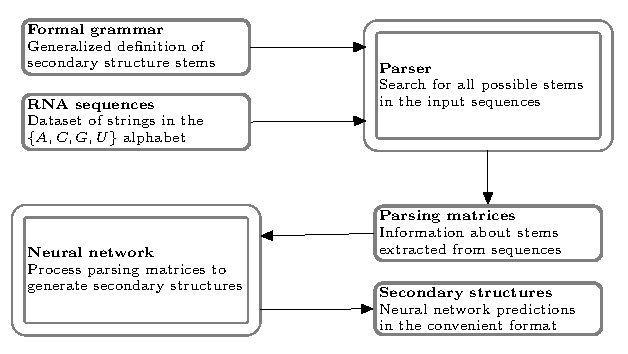
\includegraphics[width=\textwidth]{pics/arch.pdf}
\caption{Global solution architecture}
\label{arch}
\end{figure}

\subsection{Formal Grammar}
As it was mentioned before, our approach employs formal grammar not for modeling the whole structure, but for encoding its simple constructional elements (stems), therefore this grammar does not require probabilistic rules --- probability estimation is to be done by neural networks. We do not strictly fix the grammar and it can be modified in accordance with research purposes or data characteristics, so, the grammar presented below is just a concrete example that showed quite successful results during the experiments.

In figure~\ref{gram} context-free grammar $G_0$ that we use in this work as well as in the previous ones is presented. This grammar describes the recursive compositions of stems having height at least 3 (lines \textbf{7-12}) and loop size from 1 up to 20 (line \textbf{3}). Note that these constants are not mandatory and might be defined experimentally for each task. Also, $G_0$ allows only four classical nucleotides (line \textbf{4}) and conventional base pairs (line \textbf{5}), because adding the rules for more pairs and nucleotides complicates the grammar unacceptably in the context of performance, moreover, context-free grammars cannot explicitly express pseudoknots, therefore, we expect the neural network to handle all these features instead. Also, we consider only stems of height three or more (lines \textbf{1-2}), because including shorter stems would overload the parsing matrix with too much extra information. So, by this rules, a sequence folds to stem if and only if it is derivable from start nonterminal $start$ of $G_0$ (line \textbf{1}).

\begin{figure}[ht]
\begin{Verbatim}[numbers=left,xleftmargin=5mm]
start: stem3<s0>
s0: loop | loop stem3<s0> s0
loop: nucl*[1..20]
nucl: A | U | C | G
stem1<s>: A s U | G s C | U s A | C s G
stem2<s>: stem1<stem1<s>>
stem3<s>: 
      stem1<stem2<s>>
    | A stem3<s> U
    | U stem3<s> A
    | C stem3<s> G
    | G stem3<s> C
\end{Verbatim}
\caption{Context-free grammar $G_0$ for RNA secondary structure stems description}
\label{gram}
\end{figure}

Having a grammar, we want to find all the subsequences of some given sequence that may fold to stems and this is to be done by means of parsing. Formally, the result of a matrix-based parsing algorithm for an input string $w$ is an upper-triangular boolean matrix $M_P$, where $M_P [i,j] = 1$ if and only if the substring $w[i,j]$ is derivable from grammar start nonterminal. From the practical point of view, this means that parsing matrix contains one in a cell if and only if a correspondent substring folds to stem according to the rules of a given grammar, so, each stem results in a diagonal chain of ones in the matrix, because if sequence $w_1...w_n$ is a stem than it is clear that $w_2...w_{n - 1}$ is a stem, $w_3...w_{n - 2}$ is a stem and so on while the stem height is at least 3.

In figure~\ref{pars_res} we provide the parsing result for a short RNA sequence and show how parsing matrix maps with secondary structure stems. Each one cell describes the stem of height at least 3, so, this sequence contains two subsequences that may fold to stems of the first nesting level. These stems expected hydrogen bonds along with corresponding matrix cells are painted in two different colors. All nucleotide bonds forming a stem of height three or more are represented by solid lines, moreover, it is obvious that each stem of height three encapsulates stems of heights two and one which are highlighted by dotted lines. Note that these stems interfere with each other, thereby, secondary structure cannot contain both of them at the same time. So, the parsing matrix for a sequence describes all the theoretically possible folds there, but at the current step, we cannot know which one of them would be presented in the real secondary structure. Moreover, $G_0$ has certain limitations, such as stem height, loop size, and possible base pairs, so, some of the required stems may be missing in the parsing matrix. While creating a grammar we were guided by two competing ideas: to cover as many types of stems as possible and to stay with an adequate amount of extra information in the parsing matrix along with acceptable time costs for parsing.

\begin{figure}[h]
\centering
\valign{#\cr
  \hbox{%
    \begin{subfigure}[b]{.6\textwidth}
    \centering
    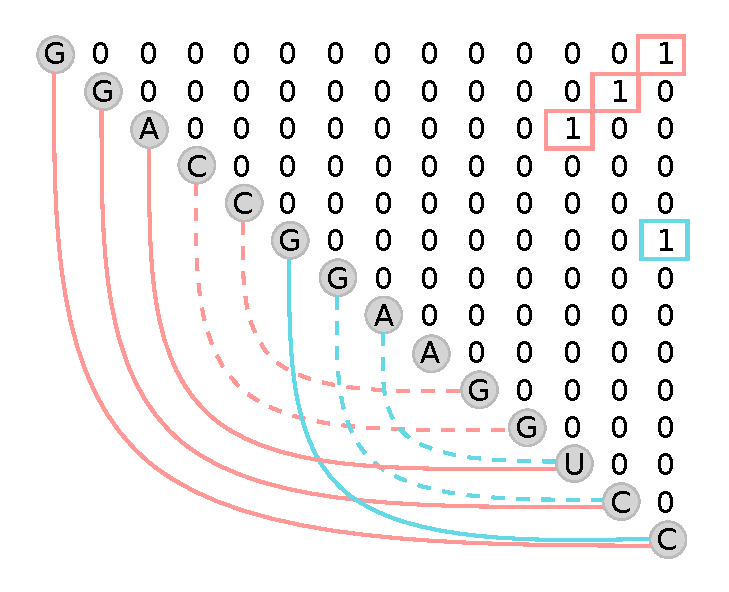
\includegraphics[width=\textwidth]{pics/matrix.pdf}
    \caption{Parsing matrix}
    \label{mtrx}
    \end{subfigure}%
  }\cr
  \noalign{\hfill}
  \hbox{%
    \begin{subfigure}{.4\textwidth}
    \centering
    \vspace{2mm}
    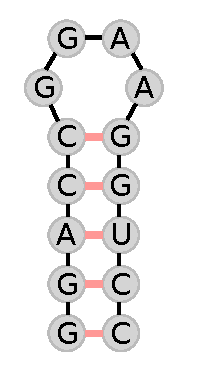
\includegraphics[width=.3\textwidth]{pics/stem1.pdf}
    \caption{First stem}
    \label{stem1}
    \end{subfigure}%
  }\vfill
  \hbox{%
    \begin{subfigure}{.4\textwidth}
    \centering
     \vspace{-2mm}
    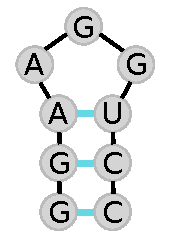
\includegraphics[width=.3\textwidth]{pics/stem2.pdf}
    \caption{Second stem}
    \label{stem2}
    \end{subfigure}%
  }\cr
}
\caption{Stems extracted from RNA sequence by parser}
\label{pars_res}
\end{figure}

Let us consider pseudoknotted structures processing. Even though it is clear that pseudoknot is not explicitly expressed in $G-0$, as well as in any context-free grammar, it consists of two stem-loop structures having half of one stem located between two halves of another, so, each of these stems separately can be derived by the rules of $G_0$. Therefore, pseudoknots will be reflected in the parsing matrix, and handling them becomes an additional task for a neural network. In figure~\ref{pk} an example of simple pseudoknot along with corresponding parsing result is provided. Two stems of this pseudoknot are highlighted with two different colors and it can be seen that all the related nucleotide bonds are presented in the parsing matrix, although at this point it is not determined whether this sequence contains a pseudoknot or it just has two possible folds in terms of grammar.

\begin{figure}[h]
\centering
\begin{subfigure}{.3\textwidth}
  \centering
  \hbox{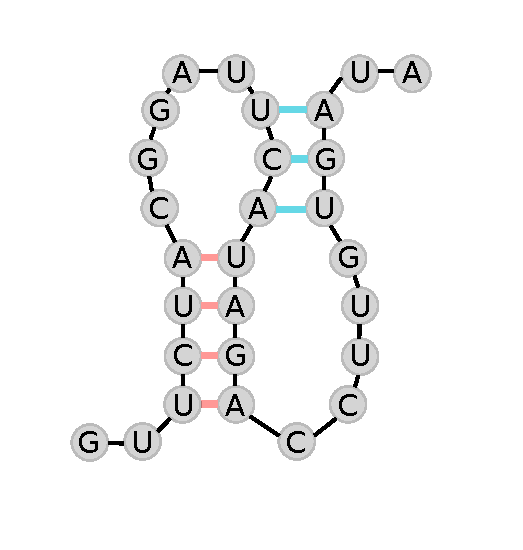
\includegraphics[width=.9\linewidth]{pics/pk.pdf}}
  \caption{Pseudonkot}
  \label{pk_a}
\end{subfigure}%
\begin{subfigure}{.7\textwidth}
  \centering
  \hbox{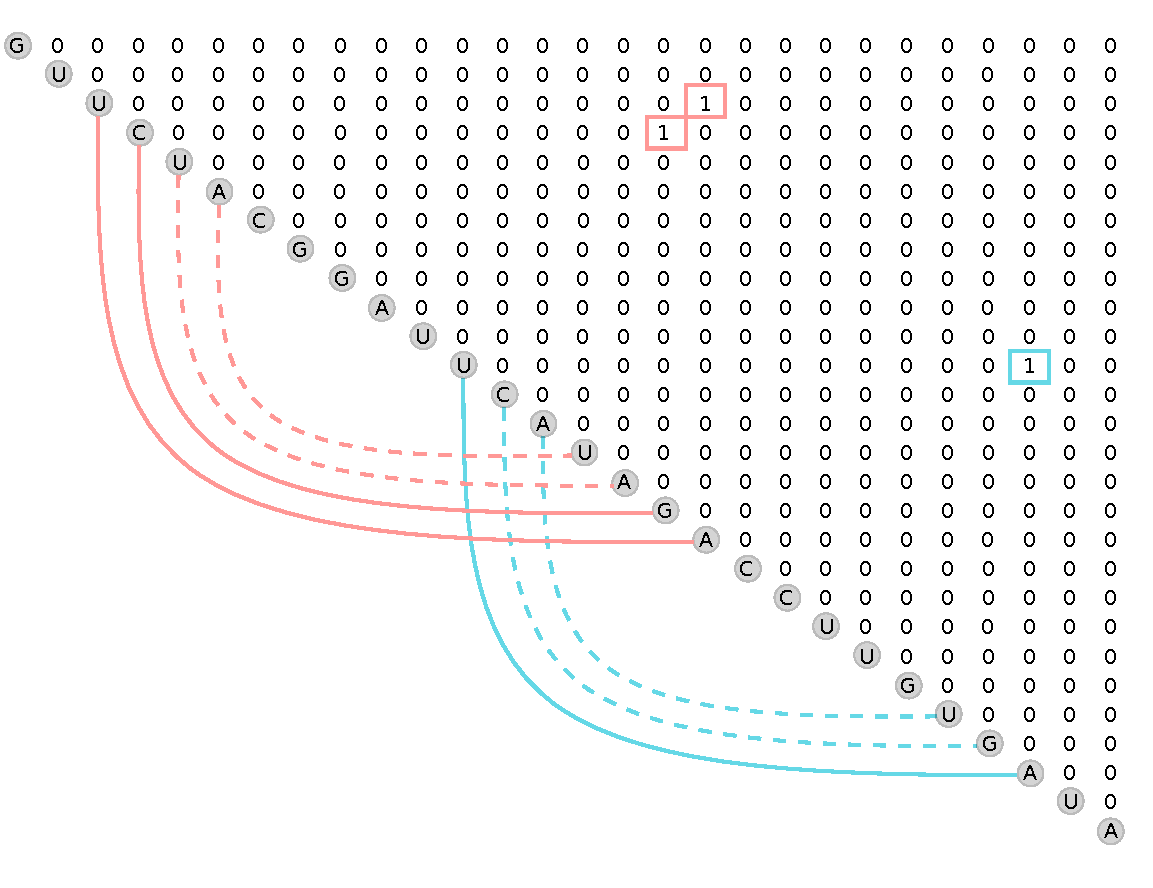
\includegraphics[width=.9\linewidth]{pics/matrix_pk.pdf}}
  \caption{Parsing matrix}
  \label{pk_b}
\end{subfigure}
\caption{Pseudoknots processing in terms of $G_0$}
\label{pk}
\end{figure}

To sum up, our grammar explicitly or implicitly describes a wide range of secondary structure elements and even the missing ones do not become a problem for our approach --- neural network is still capable to handle them. We think of such flexibility as one of the key advantages of our solution.

\subsection{Neural Network}
The matrix that our parser produced for some sequence and fixed grammar should be processed by a neural network in order to achieve a maximal similarity with the expected secondary structure for this sequence. Therefore, we need to specify the data preparing pipeline and describe the required architecture for the problem at hand. It should be noted that these are global and permanent aspects in the context of current work, however, both of them can and probably will be changed while conducting some different research.

\subsubsection{Data}
The input data for neural network (parsing matrices) was described in the previous section and now let us define the reference data source and format. There are specialized biological databases containing RNA chains of various organisms along with their secondary structures obtained by reliable methods, and such data is known to be the best for algorithms training and validation. These databases may store data using different representations (dot-bracket, connectivity table, and others), so, we need to choose a format that is convenient for our experiments and compatible with others.

One of the ways of RNA secondary structure formal representation is so-called contact map, which for an input string $w$ is a boolean matrix $M_C$, where $M_C [i,j] = 1$ if and only if nucleotides in positions $i$ and $j$ form a hydrogen bond (or, to put it simply, a contact) in secondary structure. Even though it is not the most popular format, contact matrix can be easily obtained from the corresponding connectivity table, moreover, there are certain tools that transform connectivity tables to dot-brackets~\cite{bellaousov2013rnastructure}, which provides the required compatibility. Let us consider for the above sequence $w$ the discussed earlier parsing matrix $M_P$ that has $M_P[i, j] = 1$ if and only ifsubsequence $w[i, j]$ folds to a stem. It is clear that the first and the last nucleotides of every stem form a contact, therefore, we can easily transfer between parsing matrix and contact map definitions and view the parsing matrix as a sort of a contact map, so, this format is convenient for our experiments. Note that if parser finds a stem of height three than we will see only one cell with $1$ in matrix, but such stem always wraps a stem of height two which wraps a stem of height one, so, we are always missing two contacts, therefore, after parsing we should set $M_P[i - 1, j + 1] := 1$ , $M_P[i - 2, j + 2] := 1$ if $M_P[i][j] = 1$, $i = 0..size(M_P), j = i + 1..size(M_P)$ for complete semantic equality of parsing and contact matrices.

So, a neural network should take parsing matrices as inputs and contact maps as desired outputs for the same set of RNA sequences. For convenience, we transform both matrices to black-and-white images by replacing zero cells with black pixels and one cells with white pixels. Also, we code RNA sequence at the input image main diagonal by four types of gray pixels corresponding to the four possible nucleotides in case the chain itself contains any important information about secondary structure formation patterns.

In figure~\ref{struc} we provide two-dimensional secondary structure visualization for RNA sequence along with neural network input and reference images that were made from parsing and contact matrices respectively. Contacts belonging to the three stems presented in this sequence are highlighted with three different colors in all pictures (so, input and reference images are actually grayscale, colored pixels are only here for clarification). It can be seen that not all of the stems found by the parser are presented in the real secondary structure. Moreover, the parsing result is missing several contacts since they were formed by non-canonical nucleotide pairs $A-G$ that are not expressed by grammar $G_0$. Now the purpose of a neural network becomes clear --- it should take image~\ref{struc_b} and transform it to the image~\ref{struc_c} as accurately as possible. And the ideas behind this transformation are outlined in the next section.

\captionsetup[subfigure]{justification=centering}
\begin{figure}[h]
\centering
\begin{subfigure}{.33\textwidth}
  \centering
  \hbox{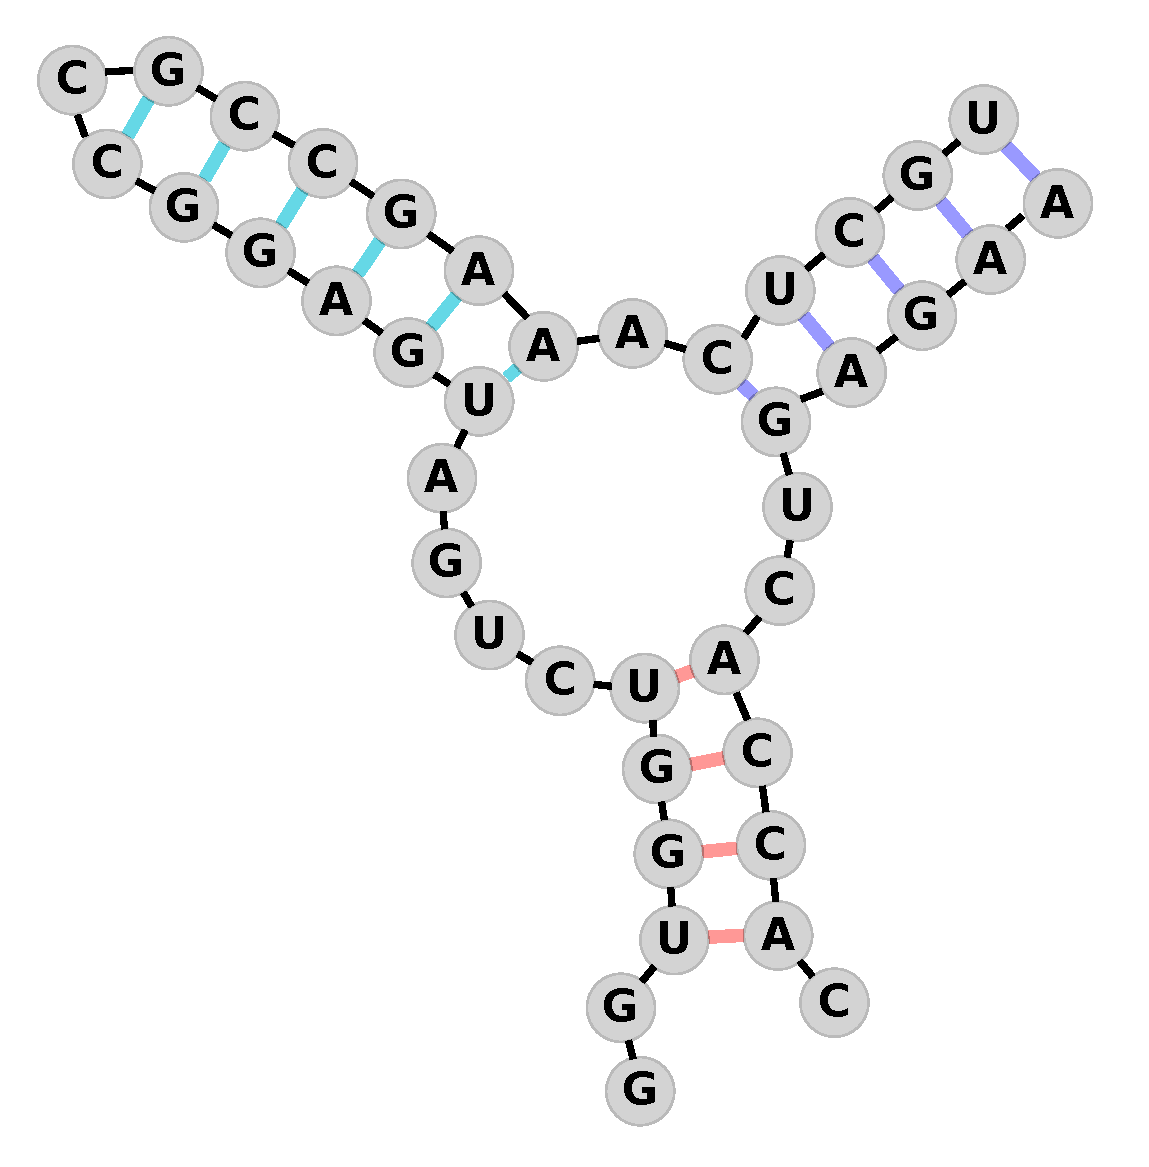
\includegraphics[width=\linewidth]{pics/struct.pdf}}
  \caption{Secondary structure visualization}
  \label{struc_a}
\end{subfigure}%
\begin{subfigure}{.33\textwidth}
  \centering
  \hbox{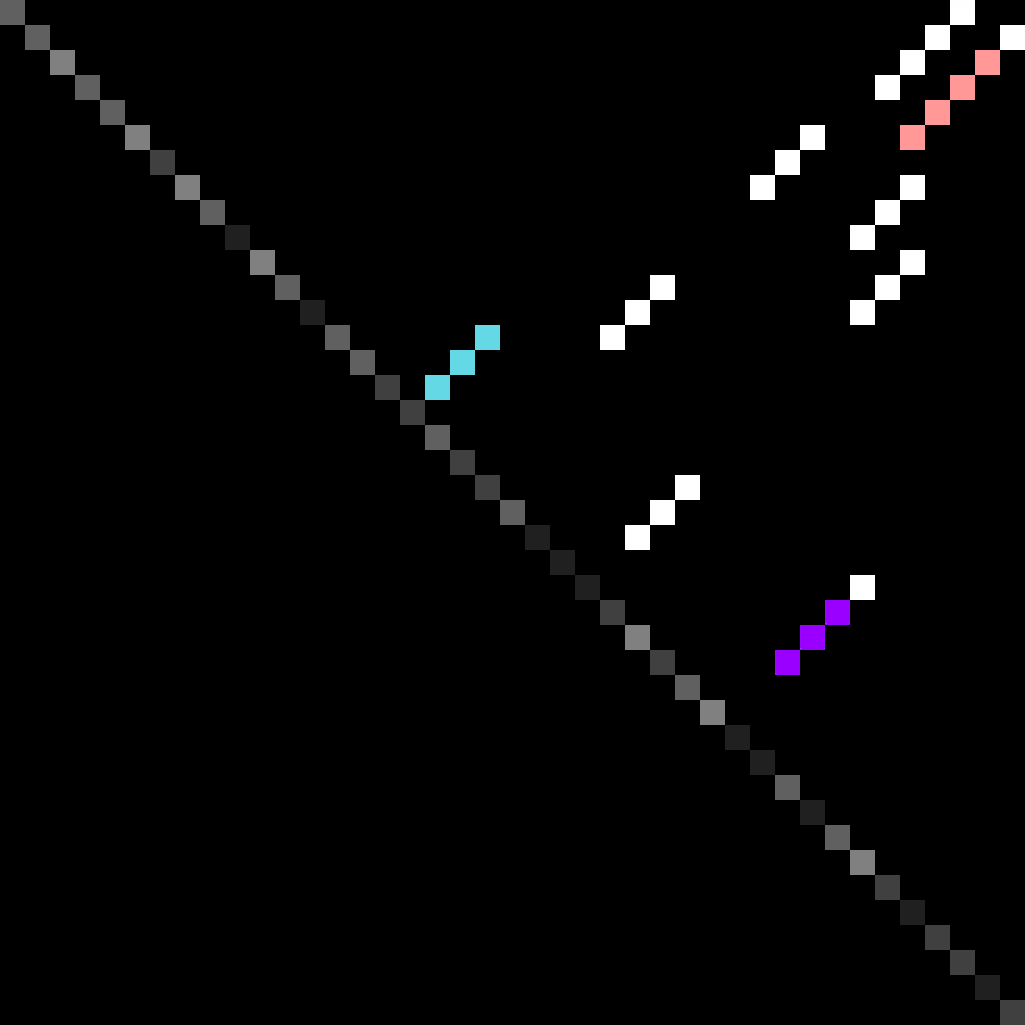
\includegraphics[width=\linewidth]{pics/in.png}}
  \caption{Input image \\ for neural network}
  \label{struc_b}
\end{subfigure}
\begin{subfigure}{.33\textwidth}
  \centering
  \hbox{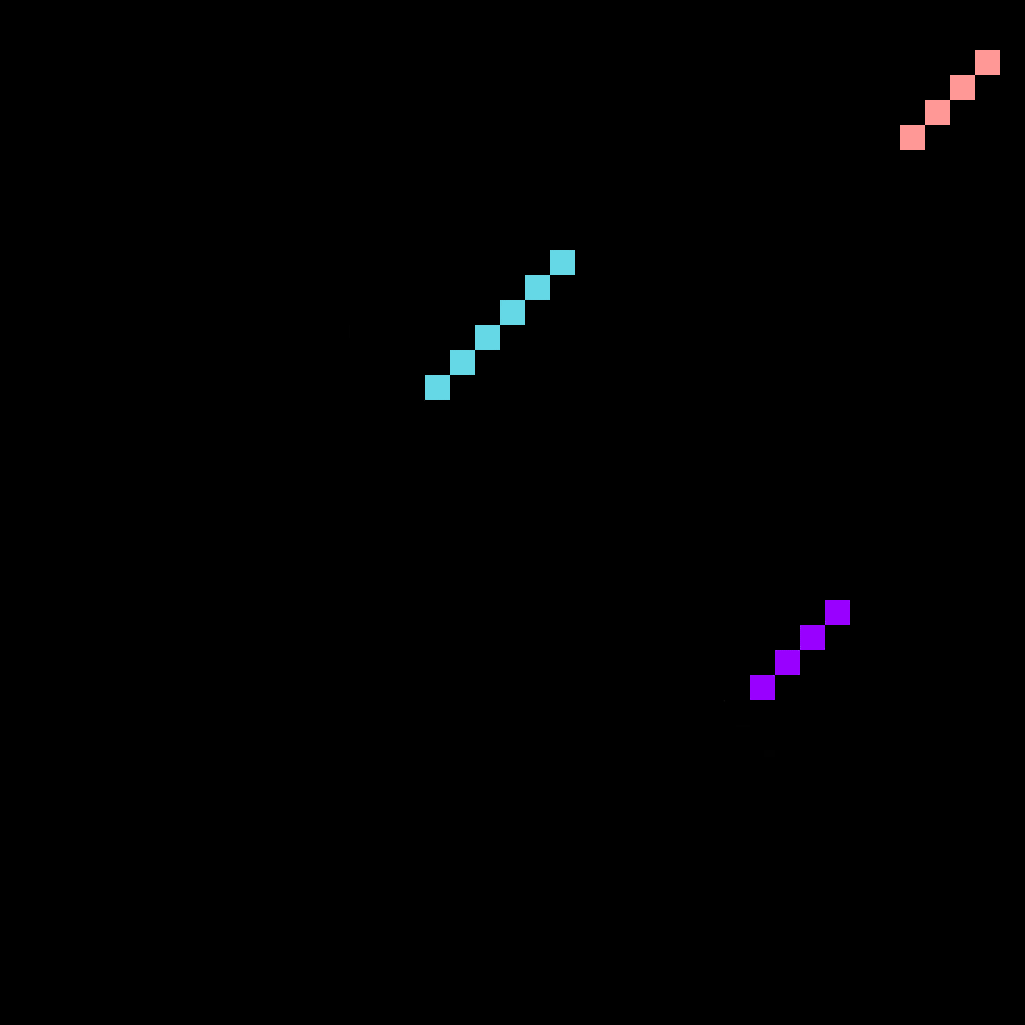
\includegraphics[width=\linewidth]{pics/out.png}}
  \caption{Reference image \\ for neural network}
  \label{struc_c}
\end{subfigure}
\caption{Secondary structure representations}
\label{struc}
\end{figure}

\subsubsection{Parallel ResNet}
One of the popular architectures for complicated images processing tasks is a residual neural network based on adding skip connections between blocks of layers~\cite{he2016deep}. ResNets solve the problem of vanishing gradient and allow to effectively use deep convolutional networks.

In this work, we developed a new architecture that showed its applicability for secondary structure prediction task during experimental research. The idea is to combine $n$ identical residual networks that take the same input, go through independent sequences of layers and connect their $n$ outputs with weighted sum hanging it over to the final residual unit that directly generates output. This parallel residual architecture along with the scheme of a typical residual unit is presented in figure~\ref{nn}, where $k$ and $n$ can be selected based on empirical evidence. We believe that the advantage of this parallel technique is that these separate networks are able to find different types of features in data and some sort of voting system allows the whole model to decide for the particular pixel whether each network behaves correctly or not.

\begin{figure}[h]
\centering
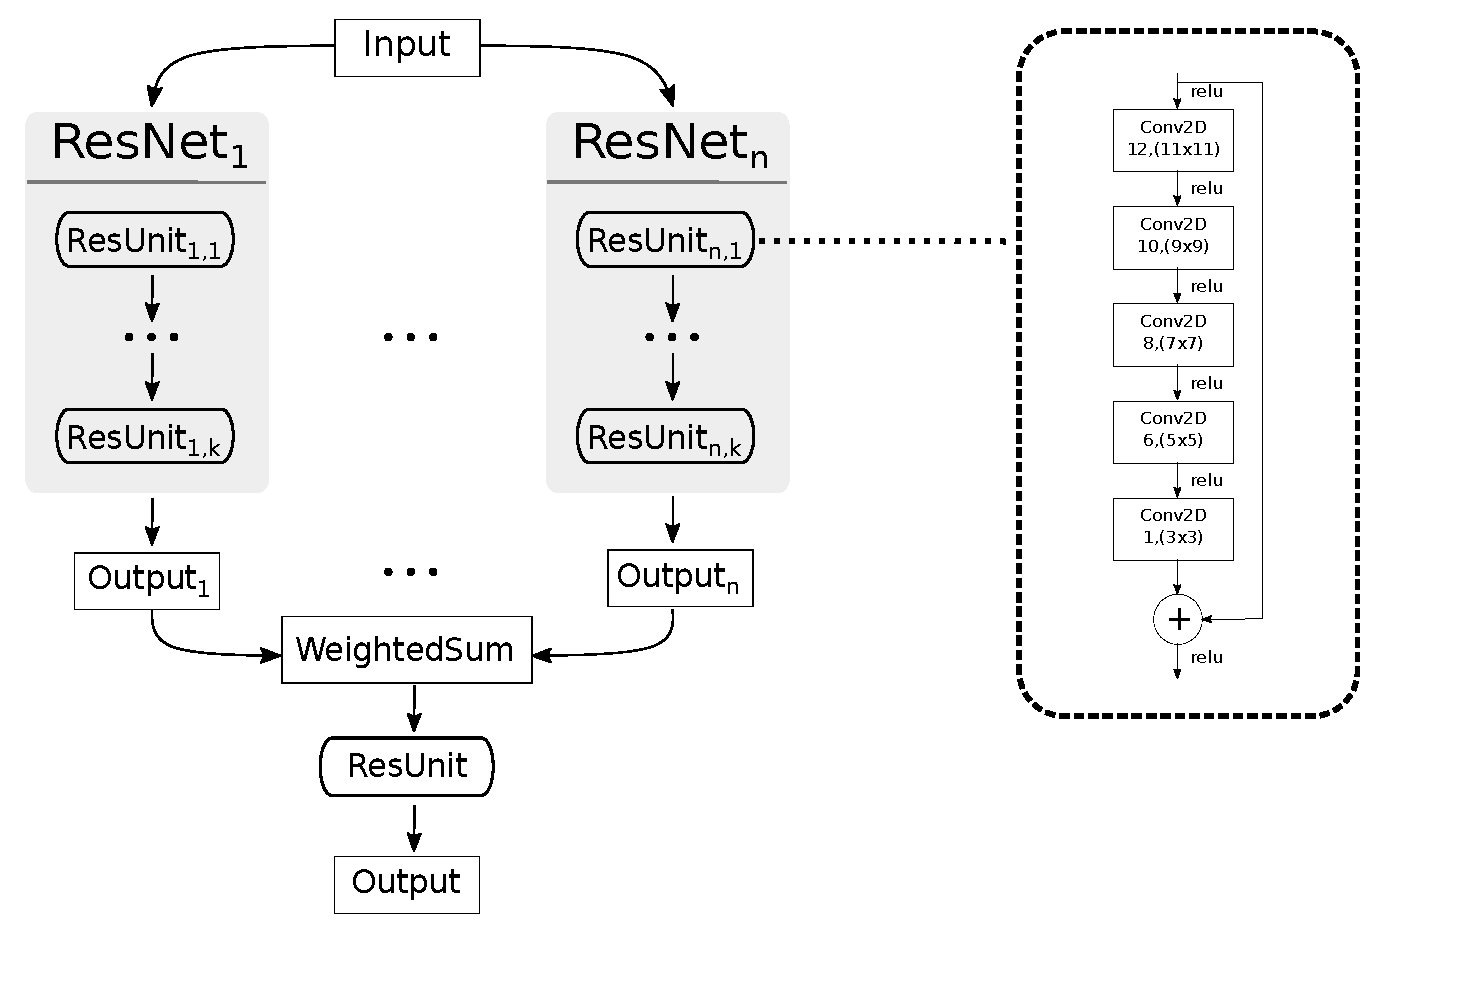
\includegraphics[width=\linewidth]{pics/nn.pdf}
\caption{Parallel ResNet architecture}
\label{nn}
\end{figure} 